\clearpage
\section{Methodology}
\label{sec:Methodology}


%%%%%%%%%%%%%%%%%%%%%%%%%%%%%%%%%%%%%%%%%%%%%%%%%%%%%%%%%%%%%%%%%%%%%%%%%%%%%%%%%%%%%%%%%%%%%%%%%%%%%%%%%%%%%%%%%%%%%%%%%%%%%%%%%%%%%%%%%%%%%%%%%%%%%%%%%%%%%%%%%%%%%%%%%%%%%%%%%%%%%%%%%%%%%%%%%%%%%%%%%%%%%%%%%%%%%%%%%%%%%%%%%%%%%%%%%%%%%%%%%%%%%%%%%%%%%%%%%%%%%%%%%%%%%%%%%%%%%%%%%%%%%%%%%%%%%%%%%%%%%%%%%%%%%%%%%%%%%%%%%%%%%%%%%%%%%%%%%%%%%%%%%%%%%%%%%%%%%%%%

\subsection{Flow Problem of Interest}
\label{sec:Flow problem of interest}
\subsubsection{Cylindrical Flow}
As a test case for running the Xcompact3d, a simple cylindrical wake case is used. In this case, the a cylinder is subjected to a flow that creates a oscillating flow behind that are commonly known as the vortex shedding phenomenon. The parameters of the cylinder is set as default, given by the input example, shown in Table \ref{tab:cyl_wake_case}.

\begin{table}[h!]
	\caption{Cylinder Wake Case Parameters}
	\centering
	\label{tab:cyl_wake_case}
	\begin{tabular}{ccccccc}
		\hline
		Re  & $x_{cyl}$ & $y_{cyl}$ & $r_{cyl}$ & $u_b$ & $\rho$ & $\nu$   \\ \hline
		300 & 5       & 6       & 0.5     & 1     & 1      & 0.0033 \\ \hline
	\end{tabular}
\end{table}

It is worth noting that the cylinder wake case is only used as a means to check the result quality of Xcompact3d case. Therefore, the cylinder wake case will not be analysed as in depth as the channel flow cases.

\subsubsection{Channel Flow}
To understand the effect of oscillating wall flow control to the effect of the flow, a case must be formulated as an example case. Generally, the case used is a canonical flow problem, which the information and data are abundantly accessible and can easily compared to one and another. Therefore, the turbulence phenomena can be thoroughly examined. In this study, a simple double periodic channel flow problem is used to be analysed for the oscillating wall flow control problem. Double periodic channel flow cases utilises periodic boundary conditions on two sets of planes: spanwise and streamwise planes. 

The first thing to do when simulating a double periodic channel flow problem is to determine the requirement of the channel flow domain size. The size of the domain must be meticulously determined to minimise the computational expenses but ensuring all of the necessary turbulence structures are captured appropriately. The minimum size of the double periodic channel flows are commonly referred as the minimal flow unit \cite{Jimenez1991}, shown in Figure \ref{fig:jimenezmfu}.

\begin{figure}[ht]
	\centering
	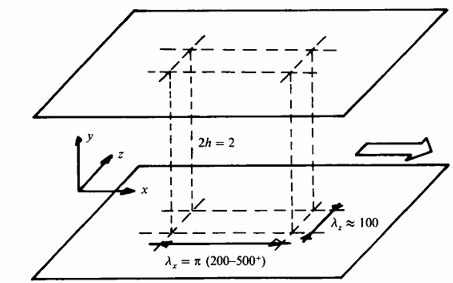
\includegraphics[width=0.6\linewidth]{Figures/JimenezMFU}
	\caption{Minimal Flow Unit of a Double Periodic Channel Flow~\cite{Jimenez1991}}
	\label{fig:jimenezmfu}
\end{figure}

\pagebreak
The length of the minimal flow unit is defined in a wall flow unit, denoted by the (+) sign. The (+) sign is a normalisation of quantities using the viscous length scale, formulated as:

\begin{equation}
	\delta_\nu = \frac{\nu}{u_\tau}
\end{equation}

Where $u_\tau$ is a function of wall friction, defined as \cite{Pope2000}:

\begin{equation}
	u_\tau = \sqrt{\frac{\tau_w}{\rho}}
\end{equation}

$\tau_w$ is related to the Reynolds numbers and the velocity gradient to the normal direction, stated as \cite{Daniel2017}:
\begin{equation}
	\tau_{w} = \frac{\partial u}{\partial y} Re
\end{equation}

$Re$ is the dimensionless number which displays the ratio between the inertial and viscous forces, expressed as \cite{NASA_Re}:
\begin{equation}
	Re = \frac{v \delta}{\nu}
\end{equation}

For study in turbulence, friction Reynolds numbers are more commonly used due to its relevance to the near wall turbulence. The equation of the friction Reynolds number is displayed below \cite{Pope2000}.
\begin{equation}
	Re_\tau = \frac{u_\tau \delta}{\nu} \approx 0.09 (2Re)^{0.88} 
\end{equation}

For the base case, the Reynolds number are defined as $Re_\tau = 180$. The quantity is chosen due to the availability of DNS channel flow data \cite{Lee2015} and the data from Xcompact3D \cite{Bartholomew2020}. The fluid properties data is shown in the Table \ref{tab:fluprop} below.

\begin{table}[ht]
	\caption{Fluid Properties}
	\label{tab:fluprop}
	\centering
	\begin{tabular}{lccccc}
		\hline
		{$\boldsymbol{Re_\tau}$} & {Re} & {$\boldsymbol{u_b}$} & {$\boldsymbol{\rho}$} & {$\boldsymbol{\nu}$} \\ \hline
		180               & 2819.294    & 1          & 1               & 0.00035        \\ \hline
	\end{tabular}
\end{table}
 



\subsection{Theoretical Background}
\label{sec:Governing equations SECTION}




\subsubsection{Governing Equations of Incompressible Fluid Flow}
\label{sec:Governing equations comp}

In a low Reynolds number case such as defined in Section \ref{sec:Flow_prob_interest}, the fluid becomes incompressible, which transforms both governing equations of the fluid flow \cite{Konoszy2024}. For the continuity equation, the expression simplifies into:

\begin{equation}
	\nabla \mathbf{u} = 0
\end{equation}

The bold variables denotes a field. For the context of $\mathbf{u}$, which is the velocity field, it can be expanded into:
\begin{equation}
	\mathbf{u} = u \mathbf{e_x} + v \mathbf{e_y} + w \mathbf{e_z}
\end{equation}

On the other hand, the momentum equation changes by dropping the compressibility term. Moreover, because of no height change involved in the channel flow, the gravity term is also dropped. Additionally, the momentum equation can be modified by normalising every term to density, as density remains constant in incompressible flow.

\begin{equation}
	\underbrace{\frac{\partial \mathbf{u}}{\partial t}}_{\rm I.} + \underbrace{(\mathbf{u}\cdot \nabla)\mathbf{u}}_{\rm II.} = - \underbrace{\frac{1}{\rho}\nabla p}_{\rm III.} + \underbrace{\nu \nabla^2 \mathbf{u}}_{\rm IV.}
\end{equation}

There are four members in a incompressible Navier-Stokes equation. The term I is the unsteady term, showing the change of the fluid velocity over time. The term II is the convective term, showing the transport of properties in the flow. The third term is the pressure gradient, showing the change of pressure in the fluid. Lastly, term IV, determines how the viscous diffusion and dissipation affecting the flow.

\subsubsection{Fractional Step Method}
\label{sec:Frac_step}
In incompressible flow, the density remains constant while the pressure changes. Therefore, the equation of state is not applicable \cite{Konoszy2024}, hence pressure and velocity equation must be calculated together in a coupled equation. In Xcompact3D, the Fractional Step Method is used \cite{Laizet2024}. In Fractional Step method, there are four steps that is conducted to couple the pressure and velocity variables \cite{Westra2002}. The first step utilises intermediate velocity field, which is expressed as \cite{vanKan1986}:
\begin{equation}
	\frac{\hat{\mathbf{u}}^{k} - \mathbf{u}^{k-1}} {\Delta t} = \gamma_{k} \mathcal{A}(\mathbf{u}^{k-1}) + \theta_{k} \mathcal{A}(\mathbf{u}^{k-2}) - \alpha_{k} \nabla p^{k-1}
\end{equation}
Where $\mathcal{A}$ is the convection-diffusion operator, which includes both terms II and IV of the Navier-Stokes equations \cite{Tamas2019}. It also worth noting that the intermediate velocity field does not satisfy the continuity equation due to its divergence-free characteristics.

Then, the second step is to solve the predicted scalar field, using the following relation:
\begin{equation}
	\nabla^2 \phi^{k} = \frac{1}{\alpha_k \Delta t}\nabla{\hat{\mathbf{u}}^k}
\end{equation}
This step is based on the pressure-Poisson equation, which makes this step computationally demanding \cite{Tamas2019}. Therefore, 3D FFT scheme is used to solve the scalar field equation \cite{Li2010}.

The third step is to update the velocity using the known scalar field and intermediate velocity field.
\begin{equation}
	\mathbf{u}^k = \hat{\mathbf{u}}^{k} - \alpha_k \Delta t \nabla \phi^{k}
\end{equation}
Finally, the pressure field is updated using the relation with the scalar field:
\begin{equation}
	p^k = p^{k-1} + \phi^k
\end{equation}


\subsubsection{Spatial Discretisation}
Solving the Navier-Stokes equation numerically requires spatial discretisation, which involves transferring the properties of the flow from one member to another \cite{Hawez2021}. Xcompact3d uses various types of compact finite difference schemes \cite{Laizet2009}, due to its ability to solve the derived values of a defined point and the neighbouring members simultaneously. This study uses the 6th-order centred Hermitian compact scheme, which solved the first derivation of the values as: \cite{Laizet2024UserGuide}:

\begin{equation}
	\alpha \mathbf{u}'_{i-1} + \mathbf{u}'_{i} + \alpha \mathbf{u}'_{i+1} = a \frac{\mathbf{u}_{i+1} - \mathbf{u}_{i-1}}{2 \Delta x} + b \frac{\mathbf{u}_{i+2} - \mathbf{u}_{i-2}}{4 \Delta x}
	\label{eq:6orderHOC}
\end{equation}

For the variables, it is set into $\alpha = 1/3$, $a = 14/9$, and $b = 1/9$ to ensure the scheme can represent a wide range of turbulence scales \cite{Laizet2009}. The second derivative also uses the 6th-order central scheme, expressed as:

\begin{equation}
	\alpha \mathbf{u}''_{j}+ \mathbf{u}''_{j+1} + \alpha \mathbf{u}''_{j+1} = a \frac{\mathbf{u}_{i+1} - 2\mathbf{u}_{i} + \mathbf{u}_{i-1}}{\Delta x^2} + b \frac{\mathbf{u}_{i+2} - 2\mathbf{u}_{i} + \mathbf{u}_{i-2}}{4\Delta x^2} + c \frac{\mathbf{u}_{i+3} - 2\mathbf{u}_{i} + \mathbf{u}_{i-3}}{9\Delta x^2}
	\label{eq:6orderHOC2nddev}
\end{equation}

To ensure the same range as the first derivative, the variables $\alpha$ is set to 2/11,  $a$ is set to 12/11, $b$ is set to 3/11, and $c$ is set to 0. Using these equations and the said variables value, the scheme can calculate the results with 4 or 5 times lower number of mesh nodes compared to 2nd order schemes while only increasing 2 times of its computational expenses \cite{Laizet2024}.




\subsubsection{Temporal Discretisation}
\label{sec:temp_disc}
Other than the spatial discretisation, temporal discretisation must also be applied to calculation so the numerical simulation can be progressed to the next time step. For nearly all of the time discretisation, the third-order Adam-Bashforth equation is used. The third order Adam-Bashforth scheme is an explicit scheme that uses one equation to progress the time step of the calculation \cite{Durran1991}, displayed as:
\begin{equation}
	\phi^{n+1} - \phi^{n} = \frac{\Delta t}{12} [23F^{n} - 16F^{n+1}+5F^{n-2}]
\end{equation}

Where
\begin{equation*}
	\begin{gathered}
		F^n = \mathbf{u}^n \phi^n\\
		F^{n-1} = \mathbf{u}^{n-1} \phi^{n-1}\\
		F^{n-2} = \mathbf{u}^{n-2} \phi^{n-2}\\
		\label{eq:Fhalf}
	\end{gathered}
\end{equation*}

For the diffusion term in the wall-normal direction, the implicit Crank-Nicolson equation is also used for the time discretisation. The temporal discretisation for the y-diffusion term can be expressed as:

\begin{equation}
	\left( \nu \frac{\partial^2 v}{\partial y^2} \right)^{n+\frac{1}{2}} = \frac{1}{2} \left( \nu \frac{\partial^2 v^{n+1}}{\partial y^2} + \nu \frac{\partial^2 v^n}{\partial y^2} \right)
\end{equation}




\subsection{Computational Procedures}
\label{sec:Computational procedures}

\subsubsection{Xcompact3d Setup}
\label{sec:Xcompact3d Setup}
Xcompact3d, as any other FORTRAN F90 based code, must be downloaded and compiled before being able to be used as an analysis software. The code is downloaded through its official Github repository, using:
\begin{verbatim}
	git clone https://github.com/xcompact3d/Incompact3d
\end{verbatim}

After that, the code is compiled using the following commands on unix, assuming 8 threads are available for compiling the code:
\begin{verbatim}
	cd Incompact3d
	export FC=mpif90
	cmake -S . -B build
	cd build
	cmake --build . -j 8
\end{verbatim}

Then by going to the \textit{input.i3d} file in each example code, the boundary conditions, as well as domain size, number of mesh, and initial condition can be changed.

%job script??? what kind of integration do you want?
 

\subsubsection{Grid Generation}
\label{sec:Gridgen}
For the entirety of the study, the cartesian structured grid is used. The entire model is discretised into a system of hexahedral-shaped elements with eight nodes connecting to each other \cite{Yeoh2010}. In a simple canonical flow as this study, the structured hexahedral grid is favoured due to the the efficiency of the shape in terms of filling the spaces, as well as the ability of minimising diffusion when transfering the properties from an element to another \cite{ANSYS2020}. Additionally, the simple connectivity of the elements makes the grid model simple to program \cite{TU2018125}.

To capture the near-wall turbulence, the size of the grid near the wall must be decreased. However, just uniformly decrease the size of the grid may cause an unnecessary computational expense as the flow on the centre of the channel flow do not have substantial gradient or turbulence structures. To compensate the problem, a stretching algorithm is introduced in the Xcompact3d program \cite{Laizet2009}, developed from \cite{Cain1984} and \cite{Avital2000}. First, the domain must be expressed in physical coordinate y and computational coordinate s.

\begin{equation}
	y = h(s), 0\le s \le 1, 0 \le y \le L_y
\end{equation}

The y-height of each members can be defined as
\begin{equation}
	h = \frac{L_y \sqrt{\beta}}{\gamma \sqrt{\alpha} \sqrt{\alpha \beta} + 1} \left\{ \tan^{-1} \left( \frac{\sqrt{\alpha \beta} + 1 \tan (\pi (\gamma s + \delta))}{\sqrt{\alpha}\sqrt{\beta}} \right) + \pi \left[ H \left( s - \frac{1 - 2\delta}{2\gamma} \right) + H \left( s - \frac{3 - 2\delta}{2\gamma} \right) \right] - \tan^{-1} \left( \frac{\sqrt{\alpha \beta} + 1 \tan (\pi \delta)}{\sqrt{\alpha} \sqrt{\beta}} \right) \right\}
	\label{eq:stretchingeq}
\end{equation}

On a default channel case in Xcompact3d, the refinement are conducted solely for the wall. Therefore, $\gamma = 1$ and $\delta = \frac12$. For all the case, $\beta$ is set to 0.259065151.



\subsubsection{Channel Flow Generalised Richardson Extrapolation Campaign}
\label{sec:GREP}
In order to conduct the Generalised Richardson Extrapolation, several channel flow models must be generated with spatial, temporal, and domain size variation. The variation of the simulation models are shown in Table \ref{tab:simmodvar}.

\begin{table}[h!]
	\centering
	\caption{Simulation Model Variation}
	\label{tab:simmodvar}
	\begin{tabular}{lcccc}
		\hline
		\textbf{Mesh Type}       & Finest    & Fine      & Medium   & Coarse   \\ \hline
		\textbf{$L_x$}              & 8$\pi$ & 4$\pi$ & 2$\pi$ & $\pi$ \\
		\textbf{$L_y$}              & 2         & 2         & 2        & 2        \\
		\textbf{$L_z$}              & 3$\pi$  & 1.5$\pi$  & 0.75$\pi$ & 0.375$\pi$ \\
		\textbf{$N_x$}              & 1024      & 256       & 64       & 16       \\
		\textbf{$N_y$}              & 1021      & 509       & 256      & 128      \\
		\textbf{$N_z$}              & 1024      & 256       & 64       & 16       \\
		\textbf{$N_{t, spinup}$}   & 35000     & 35000     & 35000    & 35000    \\
		\textbf{$N_{t, warmup}$}   & 40000     & 40000     & 40000    & 40000    \\
		\textbf{$N_{t, sampling}$} & 200000    & 50000     & 12500    & 3125     \\
		\textbf{$\Delta t$}        & 0.001     & 0.002     & 0.004    & 0.008    \\
		\textbf{$t_{tot}$}               & 200       & 100       & 50       & 25       \\ \hline
	\end{tabular}
\end{table}

Processing the result of the model variation requires a normalised resolution value so the difference in value can be consistently compared. For that, a normalised resolution is introduced as:

\begin{equation}
	NR = \frac{\Delta x_e^{current}}{\Delta x_e^{finest}} \frac{\Delta t^{current}}{\Delta t^{finest}} \frac{t_{tot}^{finest}}{t_{tot}^{current}} \frac{L_e^{finest}}{L_e^{current}}
\end{equation}

Where
\begin{equation}
	\Delta x_e = \sqrt[3]{\frac{L_x L_y L_z}{N_x N_y N_z}}
\end{equation}
\begin{equation}
	L_e = \sqrt[3]{L_x L_y L_z}
\end{equation}


\subsubsection{Oscillating Wall Generalised Richardson Extrapolation}
\label{sec:OscWall}
Simulating the oscillating wall requires a slight change to the wall boundary condition. By default, the wall is set into a no-slip condition. Therefore, the boundary condition needs to be modified so the wave equation can be included in the wall boundary condition. The base wave equation for the oscillating wall is:

\begin{equation}
	w(x, t) = A \sin(2\pi \omega t)
\end{equation}

For the ease of actuation adjustment in different Reynolds number, the wave parameters are non-dimensionalised with wall-normal values \cite{Ricco2021}. The dimensionless variables required are

\begin{equation}
	A^+ = A/u_\tau
\end{equation}
\begin{equation}
	T^+ = 2\pi \frac{u_\tau^2}{\omega\nu}
\end{equation}
\begin{equation}
	k_x^+ = k_x \frac{\nu}{u_\tau}
\end{equation}

The values of the wall-normalised parameters are based on past studies \cite{Marusic2021} \cite{Zhou2008TurbulentDR}, tabulated in Table \ref{tab:GCSset}.

\begin{table}[h!]
	\centering
	\caption{Oscillation Parameters Variation}
	\label{tab:GCSset}
	\begin{tabular}{lccccc}
		\hline
		\textbf{Re}& \textbf{$T^+_{osc}$} & \textbf{$A^+$} & \textbf{$k_x^+$}  \\ \hline
		180 & 100 & 4.9 & 0.0014 \\ \hline
	\end{tabular}
\end{table}

For the oscillating wall boundary condition problem, the code must be modified first before compiling, especially for the Navier-Stokes solver, which is named navier.f90. In the said file, the wall z-velocities \textit{uz} for both walls in \textit{pres\_correc} subroutine are changed into the defined wall wave function. In this case, the code was modified into:
\begin{verbatim}
!********NCLY==2*************************************
if (ncly1==2) then
	if (xstart(2)==1) then
		do k=1,xsize(3)
			do i=1,xsize(1)
				dpdxy1(i,k)=dpdxy1(i,k)*gdt(itr)
				dpdzy1(i,k)=dpdzy1(i,k)*gdt(itr)
			enddo
		enddo
		do k=1,xsize(3)
			do i=1,xsize(1)
				ux(i,1,k)=byx1(i,k)+dpdxy1(i,k)
				uy(i,1,k)=byy1(i,k)
				uz(i,1,k)=0.31814*sin(2*3.14159*11.18310*t)
			enddo
		enddo
	endif
endif
	
if (nclyn==2) then
	if (xend(2)==ny) then
		do k=1,xsize(3)
			do i=1,xsize(1)
				dpdxyn(i,k)=dpdxyn(i,k)*gdt(itr)
				dpdzyn(i,k)=dpdzyn(i,k)*gdt(itr)
			enddo
		enddo
	endif
	if (dims(1)==1) then
		do k=1,xsize(3)
			do i=1,xsize(1)
				ux(i,xsize(2),k)=byxn(i,k)+dpdxyn(i,k)
				uy(i,xsize(2),k)=byyn(i,k)
				uz(i,xsize(2),k)=0.31814*sin(2*3.14159*11.18310*t)
			enddo
		enddo
	elseif (ny - (nym / dims(1)) == xstart(2)) then
		do k=1,xsize(3)
			do i=1,xsize(1)
				ux(i,xsize(2),k)=byxn(i,k)+dpdxyn(i,k)
				uy(i,xsize(2),k)=byyn(i,k)
				uz(i,xsize(2),k)=0.31814*sin(2*3.14159*11.18310*t)
			enddo
		enddo
	endif
endif
\end{verbatim}

Understanding and quantifying the efficiency of the flow control method is in utmost importance for this analysis. To calculate the efficiency, the drag reduction is priorly measured using:
\begin{equation}
	DR = \frac{\tau_{w,CF} - \tau_{w,osc}}{\tau_{w,CF}} = \frac{p_{CF} - p_{osc}}{p_{CF}}
\end{equation}

For the net power saving, it is calculated using \cite{Marusic2021}:
\begin{equation}
	NPS = DR - p_{in}
\end{equation} 

Where $p_{in}$ can be calculated using:
\begin{equation}
	p_{in} = \frac{1}{p_{CF}T_{av}L_x L_y} \int_{t_i}^{t_f} \int_{0}^{L_x} \int_{0}^{L_z} W \tau_z dx dz dt
\end{equation}




